%%%%%%%%%%%%%%%%%%%%%%%%%%%%%%%%%%%%%%%%%%%%%%%%%%%%%%%%%%%%%%%%%%%%%
%
%  This is a sample LaTeX input file for your contribution to 
%  the M&C2019 topical meeting.
%
%  Please use it as a template for your full paper 
%    Accompanying/related file(s) include: 
%       1. Document class/format file: mandc.cls
%       2. Sample Postscript Figure:   figure.pdf
%       3. A PDF file showing the desired appearance: mandc2019_template.pdf
%       4. cites.sty and citesort.sty that might be needed by some users 
%    Direct questions about these files to: palmert@engr.orst.edu
%											mark.dehart@inl.gov
%
%    Notes: 
%      (1) You can use the "dvips" utility to convert .dvi 
%          files to PostScript.  Then, use either Acrobat 
%          Distiller or "ps2pdf" to convert to PDF format. 
%      (2) Different versions of LaTeX have been observed to 
%          shift the page down, causing improper margins.
%          If this occurs, adjust the "topmargin" value in the
%          physor2018.cls file to achieve the proper margins. 
%
%%%%%%%%%%%%%%%%%%%%%%%%%%%%%%%%%%%%%%%%%%%%%%%%%%%%%%%%%%%%%%%%%%%%%


%%%%%%%%%%%%%%%%%%%%%%%%%%%%%%%%%%%%%%%%%%%%%%%%%%%%%%%%%%%%%%%%%%%%%
\documentclass[letterpaper]{mandc2019}
%
%  various packages that you may wish to activate for usage 
\usepackage{tabls}
\usepackage{cites}
\usepackage{epsf}
\usepackage{appendix}
\usepackage{ragged2e}
\usepackage[top=1in, bottom=1.in, left=1.in, right=1.in]{geometry}
\usepackage{enumitem}
\setlist[itemize]{leftmargin=*}
\usepackage{caption}
\captionsetup{width=1.0\textwidth,font={bf,normalsize},skip=0.3cm,within=none,justification=centering}

%\usepackage[justification=centering]{caption}

%
% Define title...
%
\title{APPROACHES TO LOAD BALANCING \\
MASSIVELY PARALLEL TRANSPORT SWEEPS \\
 ON UNSTRUCTURED GRIDS}
%
% ...and authors
%
\author{%
  % FIRST AUTHORS 
  %
  \textbf{Tarek Habib Ghaddar$^1$, Jean C. Ragusa$^1$,Jan Vermaak$^1$, Marvin L. Adams$^1$}\\%\footnote{Footnote, if necessary, in Times New Roman font and font size 10} \\
  $^1$Dept. of Nuclear Engineering, Texas  A\&M University \\
  College Station, TX, 77843-3133 \\ 
\\
  \url{tghaddar@tamu.edu}, \url{jean.ragusa@tamu.edu}, \url{janv@tamu.edu}, \url{mladams@tamu.edu}
}
%
% Insert authors' names and short version of title in lines below
%
\newcommand{\authorHead}      % Author's names here use et al. if more than 3
           {First author}  
\newcommand{\shortTitle}      % Short title here (Shorten to fit all into a single line)
           {Paper Title }  
%%%%%%%%%%%%%%%%%%%%%%%%%%%%%%%%%%%%%%%%%%%%%%%%%%%%%%%%%%%%%%%%%%%%%
%
%   BEGIN DOCUMENT
%
%%%%%%%%%%%%%%%%%%%%%%%%%%%%%%%%%%%%%%%%%%%%%%%%%%%%%%%%%%%%%%%%%%%%%
\begin{document}
\maketitle
\justify 

\begin{abstract}
  Use 8.5$\times$11 paper size, with 1'' margins on all sides.  A required 200-250 
  word abstract starts on this line.  Leave two blank lines before ``ABSTRACT''
  and one after.  Use 11 point Times New Roman here and single 
  spacing. The abstract is a very brief summary highlighting main 
  accomplishments, what is new, and how it relates to the state-of-the-art.
\end{abstract}
\keywords{list of three to five key words}

\section{INTRODUCTION} 
Paper starts here with two blank lines before first section title.  Use 
8.5$\times$11 paper size, with 1'' margins on all sides.  Use one blank line 
before and after each subsequent section’s title.  Most of the formatting is globally
set by the specifications given in the \emph{mandc2019.cls} file.  
First-level section titles must be all uppercase and centered, and must 
be numbered in Arabic numerals as shown above.  Unlike the Word template, the body text and section titles for this \LaTeX\ template use 
11-point font.  We have found that the 11-point font in \LaTeX\ more closely 
matched the 12-point font in Word.  Introduce the topic of your work 
in this section.

The first line of a paragraph is not indented; rather add one blank line between 
paragraphs.  This is done automatically. If you are a \LaTeX\ expert you 
can likely define the established format characteristics in a more elegant 
manner than what is done here.  This is perfectly fine, so long as the 
established paper format/appearance is maintained.  This template is merely 
to assist with maintaining uniformity in paper appearance.

There are four types of reference styles: journal paper\cite{journal}, 
proceedings paper\cite{proc_paper}, book\cite{book}, and website\cite{website}.
References to websites are discouraged, but acceptable if absolutely necessary. It 
is the author’s responsibility to check links in the PDF file of your paper. 
All references should be cited in the text in numerical order, in order of 
appearance as [5-7].

The page limit for M\&C 2019 papers is 12 pages. It is strongly recommended that 
the length of any final paper should not exceed 12 pages.

\section{SECOND OR SUBSEQUENT MAJOR HEADING} 
\label{sec:first}

This is Section~\ref{sec:first}. It is followed by a subsection, that is, 
\ref{sec:second}. The style for subsection titles and all text in this template is defined 
in the \emph{mandc2019.cls} file.  Make sure to avoid widow/orphan lines.

\subsection{Subsection Title: First Character of Each Non-trivial Word is Uppercase} 
\label{sec:second}

Double-space before and after secondary titles is automatic.  Figures and 
tables should appear as close as possible to where they are first
cited, e.g., Fig.~\ref{fig:amdahl}, in the text.  Figures are numbered in Arabic 
numerals, with the caption centered below the figure, in \textbf{boldface}. For a better 
arrangement it is strongly recommended that all the figures must be placed in the``Figures'' 
folder. Triple-space before the figure, and after the figure caption.

\begin{figure}[!htb]
  \centering
  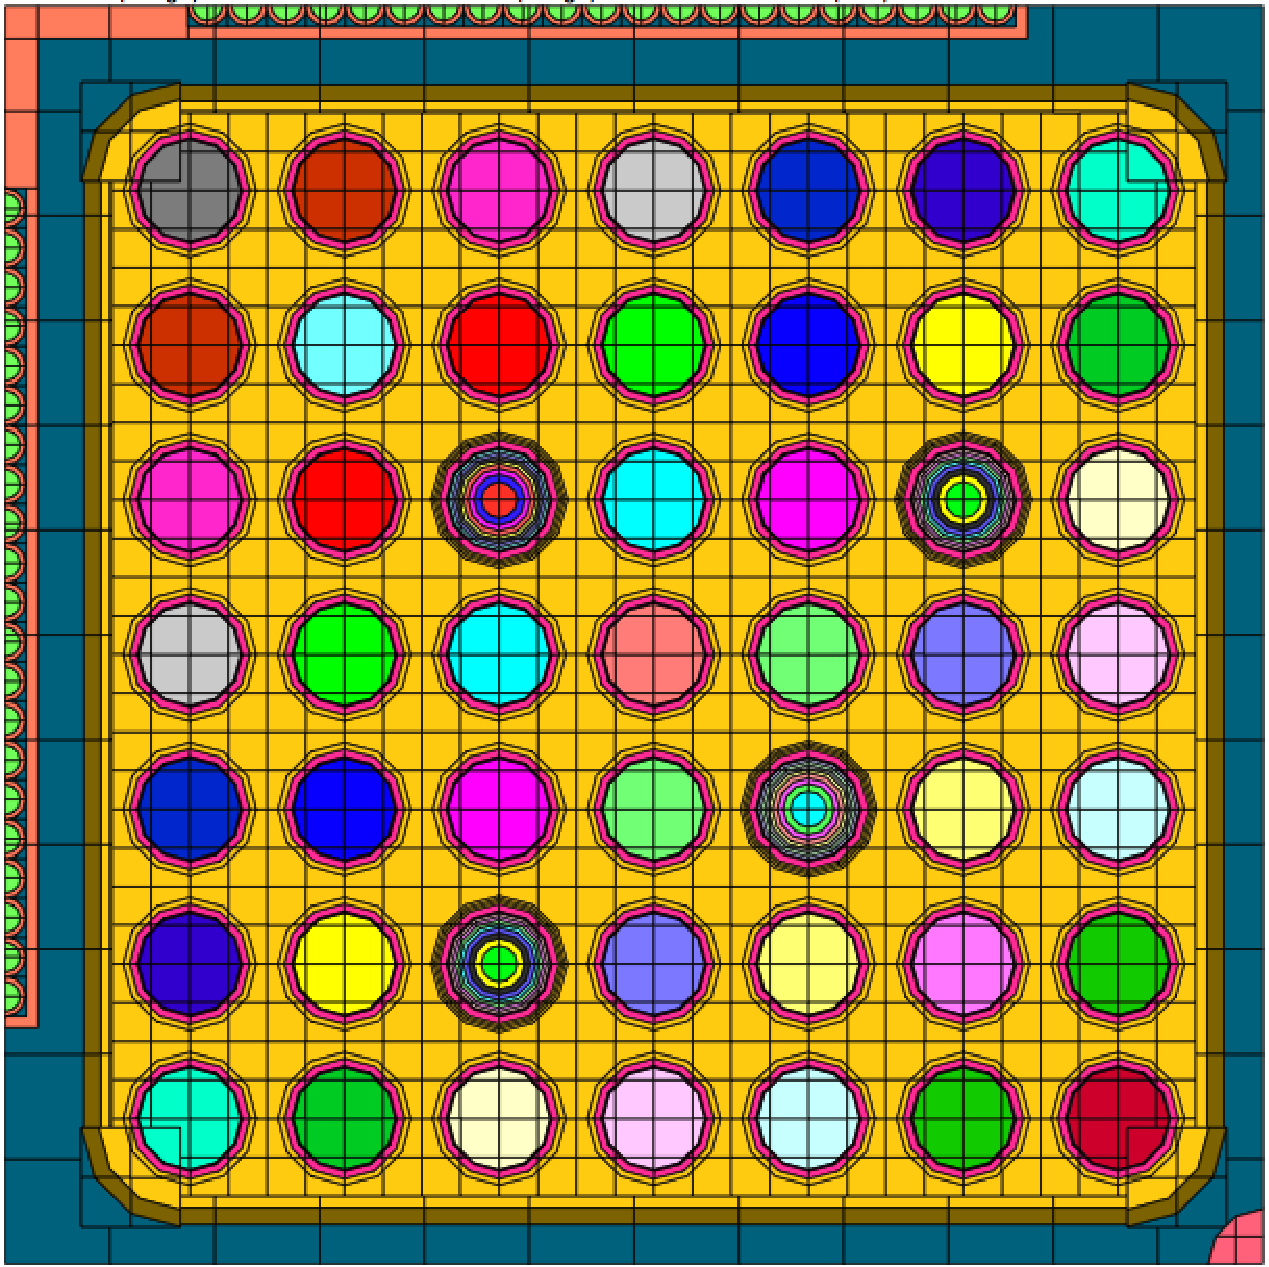
\includegraphics[scale=0.60]{./Figures/figure.pdf}
  \caption{SCALE/TRITON-NEWT Model of BWR Assembly in Order to Show and Example of a Figure and a Multi-line Caption}   
  \label{fig:amdahl}
\end{figure}

When importing figures or any graphical image please verify two things:
\vspace{-0.65cm} % THE DISTANCE BETWEEN THE ":" AND THE FIRST LINE OF THE LIST MAY VARY DEPENDING ON THE TEXT LENGTH, CHANGE THIS VALUE DEPENDING ON YOUR NEEDS.
\begin{itemize} \itemsep1pt \parskip0pt \parsep0pt
\item Any number, text or symbol is in Times font and is not smaller than 
  10-point after reduction to the actual window in your paper
\item That it can be translated into PDF
\end{itemize}

Equations, such as Eq. (\ref{sample_equation}), should be centered and 
sequentially numbered to the flush right of the formula.

\begin{equation}
  \label{sample_equation}
  \mathrm{Speedup}=\frac{1}{\frac{f}{p}+(1-f)}
\end{equation}

The continuation of a paragraph after an equation should not be indented.  
All paragraphs, as well as section or subsection headings, are separated by 
just one single empty line.

\subsubsection{Sub-subsection level and lower: only first character uppercase}

See Table \ref{table:example} for a sample table.  The ``tabls'' package is
recommended for improved row and column spacing.  Notice the caption appears 
above the table by setting the \verb!\caption! command immediately 
after the \verb!\begin{table}!. Tables are numbered in Roman 
numerals, with the caption centered above the table, in \textbf{boldface}.  
Triple-space before and after the table.

\begin{table}[!htb]
  \centering
  \caption{\bf Parallel Performance for the Sample Problem}
  \label{table:example} 
  \begin{tabular}{|c|c|c|c|} \hline 
   Number of & Wall-Clock & Speedup & Efficiency \\
   Processors & Time$^{a}$ (min) & (T$_{s}$/T$_{p}$) & (\%) \\ \hline
    \ 1 &  100.0 & \ ---    & ---  \\ \hline
    \ 2 &   52.6 & \ 1.9    & 95.0 \\ \hline 
  \end{tabular}
\end{table}

\section{CONCLUSIONS}

Present your summary and conclusions here.

\section*{NOMENCLATURE}

If variables are extensively used in the text, a Nomenclature section would be helpful to the readers.

\section*{ACKNOWLEDGEMENTS}

Acknowledge the help of colleagues and sources of funding, as appropriate.

\textbf{As an example:} The format for this template was adapted from the \LaTeX template for the PHYSOR-2018 conference posted and available on the Internet and 
most of the \LaTeX\ format definitions contained in this were already defined. The 
M\&C 2019 organizing committee deeply thank the PHYSOR-2018 technical committee 
for this great support.

% You can enter a bibliography into the document using the following format, or use the 
% bibliography style file "mandc.bst" found in the template directory.  You can use the bibliography style file
% by replacing the current bibliography block with:
% \setlength{\baselineskip}{12pt}
% \bibliographystyle{mandc}
% \bibliography{mandc}

\setlength{\baselineskip}{12pt}
\begin{thebibliography}{300}
\bibitem{journal} B. Author(s), ``Title,'' \emph{Journal Name in Italic}, 
  \textbf{Volume in Bold}, pp. 34-89 (19xx).
\bibitem{proc_paper} C. D. Author(s), ``Article Title,'' \emph{Proceedings of
  Meeting in Italic}, Location, Dates of Meeting, Vol. n, pp. 134-156 
  (19xx).
\bibitem{book} E. F. Author, \emph{Book Title in Italic}, Publisher, City \&
  Country (19xx). 
\bibitem{website} ``Spallation Neutron Source: The next-generation 
  neutron-scattering facility in the United States,'' 
  \url{http://www.sns.gov/documentation/sns\_brochure.pdf} (2002).
\end{thebibliography}

\appendix
\gdef\thesection{APPENDIX \Alph{section}}
\section{Sample Appendix 1}
\label{app:a}
If necessary, include Appendices numbered in upper case alphabetical order. This is \ref{app:a}. 



\end{document}
